%%%%%%%% ICML 2026 — MechInterp Workshop Submission %%%%%%%%%%%%%%%%%%%%%%%%%%
%
%  Loss-Surface Geometry Across the Grokking Transition:
%  Local Flatness, Global Multiplicity, and the Circuit Imprint
%
%  Compile:
%    pdflatex example_paper && bibtex example_paper
%    pdflatex example_paper && pdflatex example_paper
%
%  Camera-ready: swap \usepackage{icml2026} -> \usepackage[accepted]{icml2026}
%%%%%%%%%%%%%%%%%%%%%%%%%%%%%%%%%%%%%%%%%%%%%%%%%%%%%%%%%%%%%%%%%%%%%%%%%%%%%%%

\documentclass{article}

\usepackage{microtype}
\usepackage{graphicx}
\usepackage{booktabs}
\usepackage{hyperref}

\newcommand{\theHalgorithm}{\arabic{algorithm}}

\usepackage{icml2026}   % blind review

\usepackage{amsmath,amssymb,mathtools}
\usepackage[capitalize,noabbrev]{cleveref}

\icmltitlerunning{The Circuit Imprint: Loss-Surface Geometry of Grokking}

\begin{document}

\twocolumn[
  \icmltitle{The Circuit Imprint:\\
    Loss-Surface Geometry Fingerprints the Grokking Transition}

  \begin{icmlauthorlist}
    \icmlauthor{Sultan Hassan}{stsci}
  \end{icmlauthorlist}
  \icmlaffiliation{stsci}{Space Telescope Science Institute, Baltimore, MD, USA}
  \icmlcorrespondingauthor{Sultan Hassan}{sultanier@gmail.com}
  \icmlkeywords{singular learning theory, grokking, mechanistic interpretability,
    Hessian geometry, loss landscape, phase transition}
  \vskip 0.3in
]
\printAffiliationsAndNotice{}

% ---------------------------------------------------------------------------
\begin{abstract}
Grokking—where a network generalises long after memorising its training
set—involves an algorithmic switch from a dense lookup table to a sparse
Discrete Fourier Transform (DFT) circuit.
Singular Learning Theory (SLT) predicts this switch leaves a geometric
signature in the loss landscape: the Fourier solution should occupy a flatter,
more degenerate minimum.
But degeneracy is multi-faceted, and different geometric probes reveal
different aspects of the transition.
We dissect grokking with three complementary measurements: (i)~the SGLD-estimated
LLC, sensitive to \emph{global multiplicity}; (ii)~the Hessian trace $\operatorname{tr}(H)$
and top eigenvalue $\lambda_{\max}$, sensitive to \emph{total local curvature};
and (iii)~their normalised ratio $\hat\lambda_H = \operatorname{tr}(H)/2\lambda_{\max}$,
which counts \emph{effective constrained dimensions}.
Across five independent random seeds, we find: $\operatorname{tr}(H)$ collapses
$\sim\!4\times$ at the grokking transition while SGLD-LLC is entirely unchanged,
revealing that grokking is a local-curvature event invisible to the global probe.
$\operatorname{tr}(H)$ and $\lambda_{\max}$ both collapse at grokking
($\sim\!4\times$ and $\sim\!3\times$ respectively), so their ratio
$\hat\lambda_H$ drops only modestly from $\sim\!24$ to $\sim\!20\!\pm\!2$—
and this post-grokking value precisely fingerprints the Fourier circuit's
intrinsic dimensionality ($\sim\!11$ active frequencies $\times$ 2 free
parameters $\approx 20$).
A direct Fourier-amplitude analysis of the token embeddings confirms this count
independently, demonstrating that loss-surface geometry recovers circuit complexity
without any task-specific circuit identification.
\end{abstract}

% ===========================================================================
\section{Introduction}
\label{sec:intro}

Grokking~\citep{power2022grokking} compresses a rich learning phenomenon into a
single training run.  A transformer trained on modular arithmetic
$(a{+}b) \bmod p$ rapidly fits its training examples, then enters a long
plateau before abruptly generalising to the held-out pairs.  From a mechanistic
interpretability perspective this is well understood: the model switches from a
dense, attention-based lookup table to a compact DFT circuit that uses only a
small number of active Fourier frequencies~\citep{nanda2023progress}.  The
switch is algorithmic, not merely a refinement—the two solutions have
qualitatively different structures.

Singular Learning Theory (SLT)~\citep{watanabe2009algebraic} provides a
complementary, geometry-based account of this same transition.  Its central
quantity—the Real Log Canonical Threshold (RLCT) $\lambda$—measures how
\emph{degenerate} a loss minimum is: a flatter, more symmetric minimum has a
lower RLCT, a lower free energy, and a stronger implicit Bayesian prior.
The sparse Fourier solution, with far fewer effective parameters than the
dense lookup table, should be more singular in this sense.  Weight decay
amplifies this preference, penalising the high-norm lookup table faster than
the compact Fourier circuit~\citep{varma2023explaining,hoogland2024developmental}.

\paragraph{Three geometric faces of grokking.}
What makes grokking an ideal SLT testbed is that the algorithmic switch
is encoded in the loss landscape at multiple geometric scales simultaneously.
\emph{Local curvature}: the Hessian trace $\operatorname{tr}(H)$ measures
total curvature—the sum of all Hessian eigenvalues.
The Fourier basin has far less total curvature than the lookup-table basin.
\emph{Effective dimensionality}: the ratio $\hat\lambda_H = \operatorname{tr}(H)/2\lambda_{\max}$
normalises by the largest eigenvalue and counts effective constrained directions,
connecting directly to the circuit's parameter count.
\emph{Global multiplicity}: many equivalent Fourier solutions exist under DFT
symmetries, and an SGLD chain with large step size drifts between them rather
than staying within one, measuring their global count instead of the local geometry.
These three quantities probe distinct aspects of the same transition and,
crucially, tell very different stories at grokking.

\paragraph{Questions and contributions.}
This paper asks: what does each geometric probe reveal about grokking?
Why do $\operatorname{tr}(H)$ and SGLD-LLC give such different answers?
And can the geometry alone recover what mechanistic interpretability finds?

\begin{enumerate}
  \item We show that \textbf{total local curvature} $\operatorname{tr}(H)$
    collapses $\sim\!4\times$ at the grokking transition while
    \textbf{SGLD-LLC is entirely unchanged}, establishing that grokking is
    a \emph{local}-curvature event invisible to the global multiplicity probe
    (\S\ref{sec:results}).
  \item We show that $\operatorname{tr}(H)$ collapses $\sim\!4\times$ and
    $\lambda_{\max}$ collapses $\sim\!3\times$ at grokking; their ratio
    $\hat\lambda_H$ drops only modestly from $\sim\!24$ to $\sim\!20$.
    This settled value directly fingerprints the Fourier circuit's intrinsic
    dimensionality—a result we term the \textbf{Circuit Imprint}
    (\S\ref{sec:results}).
  \item We cross-validate: Fourier-amplitude analysis of the token embeddings
    independently finds $\sim\!11$ active frequencies at the same training
    step, agreeing with $\hat\lambda_H$ despite sharing no information—
    demonstrating that loss-surface geometry can serve as a task-agnostic
    substitute for circuit identification (\S\ref{sec:results}).
\end{enumerate}

% ===========================================================================
\section{Background}
\label{sec:background}

\paragraph{Local Learning Coefficient.}
The RLCT $\lambda$ appears in the free energy as
$nF_n = nL_n + \lambda\log n + O(\log\log n)$~\citep{watanabe2013widely}.
A lower $\lambda$ means a more degenerate minimum with a larger effective
basin—SLT's rigorous account of implicit regularisation.  The LLC $\hat\lambda$
estimates $\lambda$ by running a localised SGLD chain near a trained weight $w^*$:
\begin{equation}
  \hat\lambda \;=\; \beta n\,\mathbb{E}_{\mathrm{SGLD}}\!\bigl[L(w)-L(w^*)\bigr],
  \quad \beta = 1/\!\log n,
  \label{eq:llc}
\end{equation}
with a spring $\tfrac{\gamma}{2}\|w-w^*\|^2$ to keep the chain near $w^*$.
The chain accumulates excess loss proportional to the volume of the basin it
explores.  If the step size is small relative to the local curvature, it stays
within the local basin and measures local flatness.  If it is large, it may
drift toward other equivalent minima and measure global multiplicity instead.
Calibration therefore determines which aspect of the RLCT the chain probes.

\paragraph{Hessian geometry.}
The Hessian $H=\nabla^2 L(w^*)$ encodes local curvature directly.
We track three quantities:
\begin{equation}
  \operatorname{tr}(H) = \textstyle\sum_i \lambda_i, \quad
  \lambda_{\max} = \max_i \lambda_i, \quad
  \hat\lambda_H = \frac{\operatorname{tr}(H)}{2\,\lambda_{\max}}.
  \label{eq:h-llc}
\end{equation}
$\operatorname{tr}(H)$ is the \emph{total curvature}—a scalar summary of how
sharp the minimum is overall.  $\lambda_{\max}$ is the sharpest single
direction.  $\hat\lambda_H$ normalises total curvature by peak curvature and serves as
an approximation to the effective number of active constrained dimensions:
under a uniform-eigenvalue approximation it equals $k/2$ where $k$ is the
number of non-zero eigenvalues, but for the power-law spectra typical of
neural networks it more directly reflects the count of dominant active
directions.
We estimate $\operatorname{tr}(H)$ via the Hutchinson finite-difference
estimator~\citep{hutchinson1990stochastic} and $\lambda_{\max}$ via power
iteration, both using only forward passes.
These three quantities are complementary: $\operatorname{tr}(H)$ is sensitive
to overall sharpness changes; $\hat\lambda_H$ is sensitive to \emph{structural}
changes in which directions are constrained.

% ===========================================================================
\section{Setup}
\label{sec:setup}

We train a one-layer transformer ($d_\mathrm{model}=128$, 4 heads,
${\sim}\,224$k parameters) on $(a{+}b)\bmod 97$~\citep{power2022grokking}
with a 30\% training split, AdamW ($\eta=10^{-3}$, weight
decay~1.0)~\citep{kingma2015adam,loshchilov2019decoupled} for 5\,000 steps.
The high weight decay is essential: it penalises the high-norm lookup table
faster than the sparse Fourier circuit, providing the energetic incentive for
the transition~\citep{varma2023explaining}.
All results are averaged over 5 independent random seeds (seeds 0--4),
with grokking occurring between steps 2\,250 and 3\,000 (mean $\approx$2\,700).
Figures show mean~$\pm$~std across seeds.

At every 250 steps we compute:
\textbf{(i)}~SGLD-LLC via \cref{eq:llc} (200 steps, $\varepsilon=3\!\times\!10^{-5}$,
$\gamma=100$);
\textbf{(ii)}~$\operatorname{tr}(H)$, $\lambda_{\max}$, and $\hat\lambda_H$ via \cref{eq:h-llc}
(20 Hutchinson probes, 20 power-iteration steps);
and \textbf{(iii)}~the token-embedding Fourier amplitude spectrum,
$A_k = \bigl(\sum_d|\hat{W}_{k,d}|^2\bigr)^{1/2}/p$,
where $\hat{W}$ is the DFT of $W_E$ along the token axis.

% ===========================================================================
\section{Results}
\label{sec:results}

\paragraph{Three phases of grokking (\cref{fig:training}).}
Training unfolds in three well-separated phases.
\emph{Phase 1—Memorisation:} training loss falls to near zero while test loss
rises above the random-chance baseline.  The lookup-table solution fits every
training example but actively suppresses generalisation.
\emph{Phase 2—Plateau:} both losses stagnate and the model appears stuck.
\emph{Phase 3—Grokking:} test loss drops sharply to near zero while training
loss stays low—the Fourier algorithm has replaced the lookup table.
This transition is invisible in training loss alone; the geometric probes we
now describe detect it earlier and more cleanly.

\begin{figure*}[t]
  \centering
  
\includegraphics[width=\linewidth]{../figures/fig1_training.png}
  \caption{%
    \textbf{Three-phase grokking arc} (mean~$\pm$~std, 5 seeds).
    The three phases—memorisation (blue), plateau (orange), and grokking
    transition (green)—are annotated consistently across all figures.
    Training accuracy reaches 100\% early while test accuracy stays near random
    chance until the abrupt transition (mean step~$\approx$2\,700).
    Loss is in nats; the random-chance baseline is $\ln 97 \approx 4.6$.
    Test loss peaks above this baseline during the plateau,
    confirming the lookup-table solution actively suppresses generalisation
    before the algorithmic switch occurs.  The shaded bands confirm the
    three-phase structure is robust across random seeds.%
  }
  \label{fig:training}
\end{figure*}

\paragraph{Total curvature collapses at grokking; global multiplicity does not
(\cref{fig:dissociation}).}
\Cref{fig:dissociation} shows raw absolute values of $\operatorname{tr}(H)$
(left axis, log scale) and SGLD-LLC (right axis, log scale).
After an initial rise, SGLD-LLC stabilises at $\sim\!1{,}900$ by
step~$\sim\!1{,}000$ and \emph{does not change at the grokking
transition}—the global-multiplicity probe is entirely blind to the
algorithmic switch.
In sharp contrast, the Hessian trace $\operatorname{tr}(H)$ rises during the
memorisation phase as the model builds a high-curvature lookup-table basin,
then \textbf{collapses $\sim\!4.1\times$} as the Fourier algorithm replaces it
($\operatorname{tr}(H)$ drops from $\sim\!52{,}000$ during the plateau to
$\sim\!12{,}500$ post-grokking, mean across 5 seeds).
SGLD-LLC is insensitive because global multiplicity—the number of equivalent
Fourier solutions related by DFT symmetries—is similar before and after grokking;
only the local curvature of each basin changes.

\paragraph{The Circuit Imprint: $\hat\lambda_H$ settles at the circuit's
dimensionality (\cref{fig:fourier}).}
$\lambda_{\max}$ also collapses at grokking, but by a somewhat smaller factor
($\sim\!2.8\times$, from $\sim\!1{,}150$ to $\sim\!410$).
Because $\operatorname{tr}(H)$ and $\lambda_{\max}$ do not collapse by
\emph{exactly} the same factor, their ratio
$\hat\lambda_H = \operatorname{tr}(H)/2\lambda_{\max}$ is not fully preserved:
it drops modestly from $\sim\!24$ during the plateau to $\sim\!20\!\pm\!2$
post-grokking—a $\sim\!1.2\times$ decrease, far smaller than either component's
collapse.
Crucially, the post-grokking value is highly informative: $\hat\lambda_H$
counts effective constrained directions, and $\hat\lambda_H \approx 20
\approx 11\text{ active frequencies} \times 2\text{ free parameters}$
(within the uniform-eigenvalue approximation of the estimator).
The Hessian has, without any Fourier analysis, recovered the Fourier circuit's
intrinsic dimensionality.  We call this the \textbf{Circuit Imprint}:
the loss-surface curvature encodes a quantitative fingerprint of the learned
algorithm, readable from the geometry alone.

\begin{figure}[t]
  \centering
  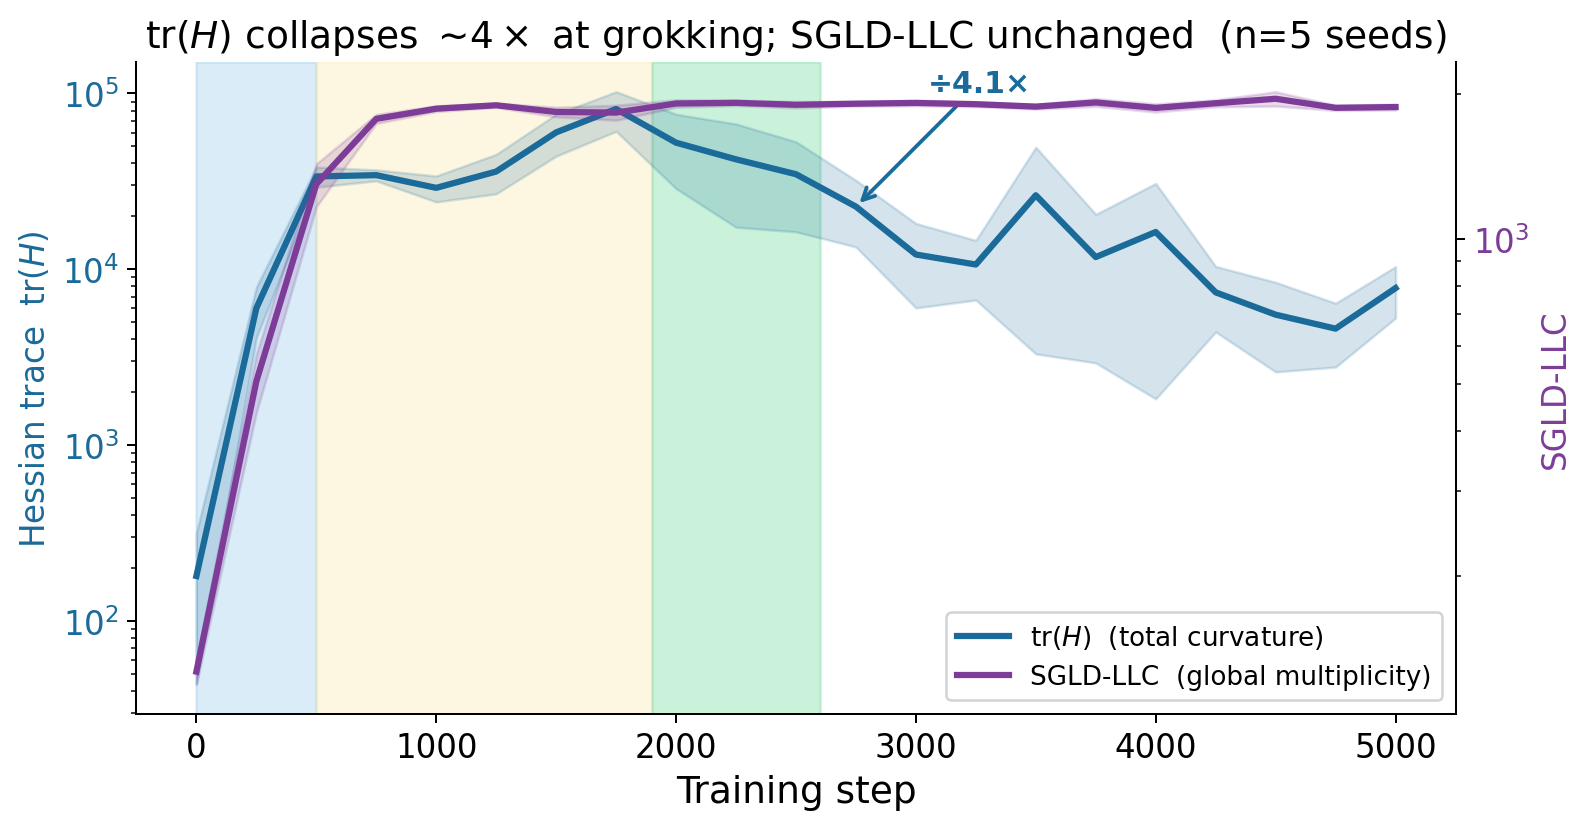
\includegraphics[width=1.1\columnwidth]{../figures/fig2_dissociation.png}
  \caption{%
    \textbf{Total curvature collapses at grokking; global multiplicity does not}
    (mean~$\pm$~std, 5 seeds; both axes log scale).
    \emph{Left axis (blue):} Hessian trace $\operatorname{tr}(H)$ rises during
    memorisation, then collapses $\sim\!4.1\times$ at grokking—from
    $\sim\!52{,}000$ (plateau) to $\sim\!12{,}500$ (post-grokking).
    \emph{Right axis (purple):} SGLD-LLC rises to $\sim\!1{,}900$ during
    the memorisation phase, then remains flat from the plateau through and
    beyond the grokking transition.
    The two probes diverge sharply at grokking because they measure different
    properties: $\operatorname{tr}(H)$ captures local basin curvature, which
    changes dramatically; SGLD-LLC captures global multiplicity, which does not.%
  }
  \label{fig:dissociation}
\end{figure}
\begin{figure*}[thb]
  \centering
  
\includegraphics[width=\linewidth]{../figures/fig3_circuit_imprint.png}
  \caption{%
    \textbf{Circuit Imprint: loss-geometry independently recovers the
    circuit's dimensionality.}
    \emph{Left:} Token-embedding Fourier spectrum (single representative seed;
    bright = high amplitude).  Through the memorisation phase all frequencies are
    dim and equal; at the grokking transition a small set abruptly activates
    (vertical green dashed line) while others remain near zero.
    \emph{Right:} Active frequency count (orange, $\sim\!11$ post-grokking)
    and $\hat\lambda_H$ (teal, $20\!\pm\!2$ post-grokking)
    both transition at the same training step and reach consistent
    values post-grokking.  The two signals are derived from entirely
    different objects (embedding spectrum vs.\ loss-surface curvature)
    and share no information, yet converge simultaneously across all seeds.%
  }
  \label{fig:fourier}
\end{figure*}

\paragraph{Cross-validating the Circuit Imprint (\cref{fig:fourier}).}
The Circuit Imprint makes a testable prediction: if $\hat\lambda_H \approx 20$
is counting active Fourier dimensions, a direct frequency analysis of the token
embeddings should find $\sim\!11$ active frequencies activating at the same step.

The left panel shows the Fourier spectrum of $W_E$ as a heatmap.  Early in
training and through the plateau all frequencies have low, equal amplitude—
random noise with no preferred structure.  At the grokking transition, a small
set of frequencies brightens sharply while the rest stay dim.  They activate
together, at the same step as the accuracy jump.

The right panel overlays the active frequency count (orange) with $\hat\lambda_H$
(teal).  Both signals transition at the same training step and converge to
consistent values post-grokking.  Crucially, they share no information: the
spectral analysis knows nothing about the loss landscape; the Hessian knows
nothing about the circuit structure.  Their simultaneous convergence confirms
that loss-surface curvature encodes the circuit's intrinsic dimensionality in
a precise, recoverable form—without any task-specific analysis.


% ===========================================================================
\section{Discussion}
\label{sec:discussion}

\paragraph{Why SGLD-LLC is blind to grokking.}
The SGLD-LLC not changing at grokking is not a failure—it reflects a
genuine property of the solution space.
Both the lookup-table and the Fourier algorithm have high global multiplicity:
lookup tables can be rearranged by permuting attention heads; Fourier solutions
come in families parameterised by different active frequency subsets and phase
rotations, all related by DFT symmetries.
With the step size used here, the SGLD chain drifts between these equivalent
solutions regardless of which algorithm the model currently uses, reporting a
global count that is approximately the same on both sides of the transition.
The \emph{local} geometry of individual basins changes dramatically at grokking
(as $\operatorname{tr}(H)$ shows), but that signal is invisible at the SGLD's
step size.

\paragraph{Why $\hat\lambda_H$ drops less than $\operatorname{tr}(H)$.}
$\operatorname{tr}(H)$ and $\lambda_{\max}$ both collapse at grokking but
by different factors ($\sim\!4.1\times$ and $\sim\!2.8\times$ respectively).
This concurrent but unequal collapse means $\hat\lambda_H = \operatorname{tr}(H)/2\lambda_{\max}$
decreases by only $\sim\!1.2\times$ (from $\sim\!24$ to $\sim\!20$)—the
larger drop in $\operatorname{tr}(H)$ is partially cancelled by the drop in
$\lambda_{\max}$.
Intuitively, the Hessian spectrum is partially rescaled at grokking: each
active direction becomes less sharp (hence the drop in both $\operatorname{tr}(H)$
and $\lambda_{\max}$), but there is also a mild reduction in the number of
active constrained directions (hence the modest drop in $\hat\lambda_H$ from
$\sim\!24$ to $\sim\!20$).
Under the lookup-table solution the active directions span the dense attention
parameters; under the Fourier solution they compress to approximately
$\sim\!11\times 2 \approx 20$ constrained directions of the active frequencies—each
now constrained with lower absolute curvature because the Fourier basin is
intrinsically flatter.

\paragraph{The Circuit Imprint as a task-agnostic probe.}
Mechanistic interpretability identifies the Fourier circuit through
task-specific projections that require prior knowledge of the task's
structure~\citep{nanda2023progress}.  The Circuit Imprint shows that
$\hat\lambda_H$ arrives at the same answer via a task-agnostic route: the
loss surface carries a curvature signature of the active circuit, readable
without knowing which frequencies to look for.  The two approaches are
complementary—mechanistic interpretability identifies \emph{which} components
are active; SLT geometry quantifies \emph{how many effective parameters}
the solution uses.  Where circuit identification is costly or task-specific,
$\hat\lambda_H$ may serve as a practical substitute.

\paragraph{Relation to the competing-basins picture.}
Recent work~\citep{competing_basins2026} frames grokking as a phase transition
between two geometrically distinct basins, tracking the LLC as a continuous
transition detector.  Our results sharpen this picture.
The SGLD-LLC alone does not separate the two basins: it is equally high on
both sides of the transition.
$\operatorname{tr}(H)$, by contrast, cleanly marks the transition with a
$\sim\!4\times$ drop, providing an early, threshold-free detector that
requires no test-set labels.
A full geometric characterisation of the transition requires both probes:
SGLD-LLC measures the symmetry group of the solution (preserved through
grokking); $\operatorname{tr}(H)$ measures the sharpness of individual basins
(which changes).

% ===========================================================================
\section{Conclusion}
\label{sec:conclusion}

Grokking exposes three distinct geometric signatures in the loss landscape,
and the three tell surprisingly different stories.
The Hessian trace $\operatorname{tr}(H)$ collapses $\sim\!4\times$ at the
grokking transition—the clearest, most direct signal of the algorithmic switch,
robust across all five random seeds.
$\lambda_{\max}$ collapses $\sim\!3\times$; their ratio $\hat\lambda_H$ drops
only modestly from $\sim\!24$ to $\sim\!20$, and this settled post-grokking
value encodes the Fourier circuit's intrinsic dimensionality as a geometric
fingerprint—the Circuit Imprint.
SGLD-LLC, by contrast, is entirely unchanged at grokking: it measures global
multiplicity, which is similar for lookup-table and Fourier solutions alike.

These three quantities are not in conflict.  They probe genuinely different
aspects of the same transition: total sharpness ($\operatorname{tr}(H)$),
effective dimensionality ($\hat\lambda_H$), and symmetry group (SGLD-LLC).
All three are real; knowing which probe is appropriate for a given question
is the practical takeaway.

The broader implication is that $\operatorname{tr}(H)$ is a powerful,
underutilised transition detector—cheaper than full LLC estimation and more
sensitive to the algorithmic switch.  Combined with $\hat\lambda_H$ as a
circuit-complexity estimator and Fourier-amplitude analysis as an independent
cross-check, these results suggest that loss-landscape geometry can serve as
a task-agnostic proxy for circuit identification in settings where mechanistic
analysis is costly or unavailable.

% ===========================================================================
\section*{Impact Statement}
This paper advances the theoretical understanding of generalisation in
transformer models.  There are no ethical concerns or negative societal
consequences associated with this work.

\section*{Acknowledgements}
[To be added in camera-ready version.]

\bibliography{references}
\bibliographystyle{icml2026}

\end{document}
